\documentclass{article}
\usepackage[utf8]{inputenc}
\usepackage[spanish]{babel}
\usepackage{graphicx}
\usepackage{longtable}
\usepackage{float}
\graphicspath{{./img/}}

\title{Práctica 2. Algoritmos divide y vencerás - Suma de dos elementos}

\author{Noelia Escalera Mejías \\
		\and Alejandro Menor Molinero \\
		\and Javier Núñez Suárez \\
		\and Adra Sánchez Ruiz \\
		\and Jesús Torres Sánchez}
\begin{document}
	\maketitle
	\tableofcontents
	\
	\
	\section{Introduccion}
	El objetivo de esta práctica es realizar dos algoritmos que desarrollen la siguiente tarea: partiendo de un valor inicial generado, deben buscar en una lista (en nuestro caso, usaremos un vector), dos elementos cuya suma resultante sea igual al valor inicial generado. 
	
	Los algoritmos realizados son: uno básico, que es un algoritmo fuerza bruta que compara cada componente del vector hasta encontrar dos elementos que sumen lo mismo; y otro divide y vencerás, que primero ordena el vector, y después comprueba los valores extremos recursivamente, descartando uno de ellos dependiendo del valor umbral. 
	
	
	\subsection{Eficiencia teórica: algoritmo básico}
	
	 Dado un vector de n enteros, para determinar si existen en el vector dos números cuya suma sea igual a un valor dado, el algoritmo desarrollado realiza la suma uno a uno de cada
	 elemento del vector con sus consecutivos.
	 Para ello hace uso de la anidación de dos bucles, de modo que la eficiencia de este algoritmo es de orden cuadrática $O(n^2)$.
	
	
	\subsection{Eficiencia teórica: algoritmo DyV}
	
	En este caso, para determinar si en el vector existen dos números cuya suma sea igual a un valor dado, primero se ordena dicho vector mediante el uso del algoritmo Quicksort.
	Una vez ordenado el vector, el algoritmo desarrollado de Divide y Vencerás para la suma, toma los elementos de los extremos y los suma, si el resultado de la suma es el propio elemento, lo
	devuelve. Si por el contrario el resultado es mayor que el número que buscamos, se vuelve a llamar al algoritmo de forma recursiva con el elemento de la izquierda, y el valor anterior al
	último. Y en otro caso, es decir, si el resultado es menor, se hace una llamada recursiva, esta vez con el último valor, y el siguiente del de la izquierda. Así sucesivamente hasta que se
	encuentre el valor o hasta que se haya recorrido todo el vector. Este algoritmo es de orden lineal $O(n)$.
	Como resultado, el orden de eficiencia total es el máximo de los órdenes de los dos segmentos en los que hemos dividido el problema. Como Quicksort está acotado por $O(n*logn)$ y el de
	nuestro algoritmo por $O(n)$, la eficiencia conjunta es de orden $O(n*logn)$ ya que este es el
	dominante.
	
	Además, hemos calculado la eficiencia teórica mediante el método de expansión. Este algoritmo consiste en desarrollar progresivamente la ecuación de recurrencia para diversos niveles sustituyendo cada aparición del valor de la función por la expresión que se especifica en la recurrencia. Es necesario identificar un patrón general, que en este caso hemos elegido ((n-1) + 2i) y aplicarlo para resolver.
	

	
	$T(n) = T(n-1) + C$ 
	
	\
	$T(n) = T(n-2) + 2*C$
	
	\
	$T(n) = T(n-i) + 2*i$
	
	\
	$T(n) = k + 2*(n-2)$
	
	\
	$T(n) = k + 2*n - 4$
	
	\section{Análisis de eficiencia empírica}
	Vamos a medir el tiempo que tardan en ejecutarse los dos algoritmos:
	
	\
	Además, los compararemos entre ellos cuando sea interesante hacerlo.
	
	\
	He aquí una tabla comparativa del tiempo que tarda cada algoritmo según el tamaño del vector a ordenar.
	
	
	\section{Análisis de eficiencia híbrida}
	Ajuste de los algoritmos de acuerdo a su eficiencia teórica y los datos obtenidos en la eficiencia empírica.
	
	\subsection{Ajuste del algoritmo básico}
	
	\begin{longtable}{|c|c|c|}
		\hline
		Constante		& Valor			& Error estándar	\\ \hline
		a0              & 1.12169e-09	& 0.9625 \\ \hline
		a1              & 1.10848e-07	& 100.2	 \\ \hline
		a2              & -0.000225747	& 106	 \\ \hline
	\end{longtable}
	
	\begin{figure}[H]
		\centering
		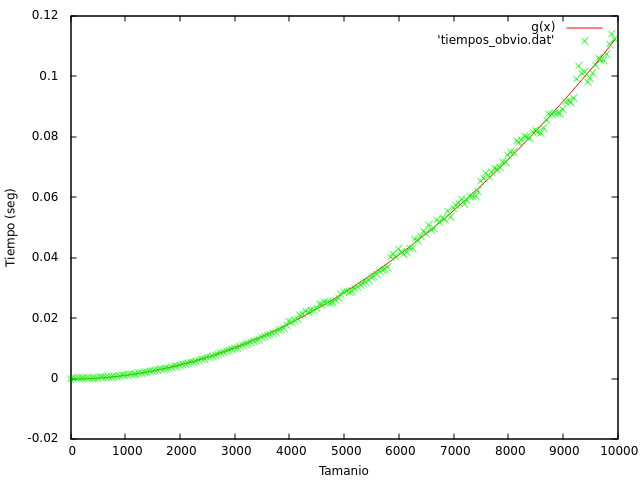
\includegraphics[totalheight=8cm]{img/Basico_ajustada}
		\caption{Ajuste algoritmo básico}
		\label{fig:Basico_ajustada}
	\end{figure}
	
	\subsection{Ajuste del algoritmo Divide y Vencerás}
	
	\begin{longtable}{|c|c|c|}
		\hline
		Constante		& Valor			& Error estándar	\\ \hline
		b0              & 7.472e-09		& 22.27	 \\ \hline
		b1              & 4.17793e-08 	& 37.34	 \\ \hline
		b2              & -6.70324e-06	& 94.89	 \\ \hline
	\end{longtable}
	
	\begin{figure}[H]
		\centering
		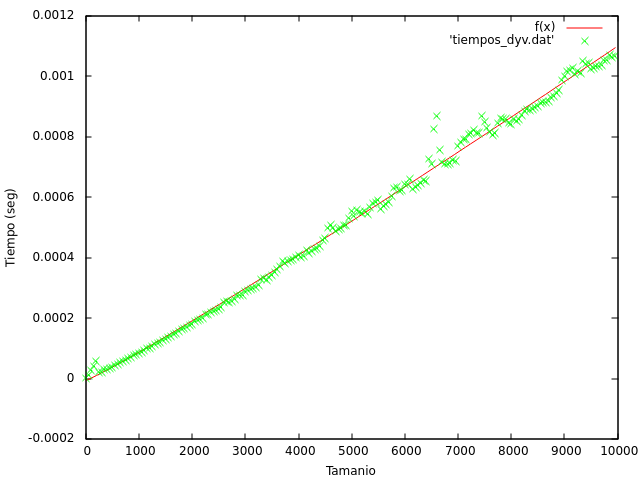
\includegraphics[totalheight=8cm]{img/DyV_ajustada}
		\caption{Ajuste algoritmo Divide y Vencerás}
		\label{fig:DyV_ajustada}
	\end{figure}
	
	Comparativas entre funciones:
	
	\begin{figure}[H]
		\centering
		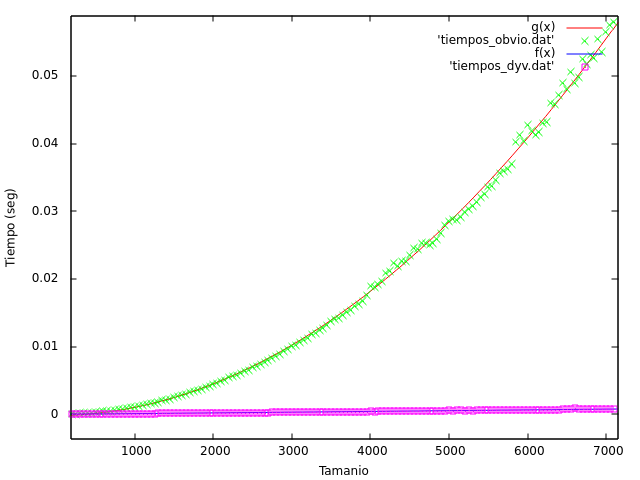
\includegraphics[totalheight=8cm]{img/ajustes_total}
		\caption{Ajustes comparativos}
		\label{fig:ajustes_total}
	\end{figure}

\end{document}
